\chapter{Multipath TCP}
\label{chap:multipathtcp}

\section{Transmission Control Protocol (TCP)}
MPTCP is an extension of regular TCP, the ubiquitous protocol for highly reliable host-to-host communication in a packet-switched computer network. A proper introduction of the fundamental of TCP is due.


TCP is a host-to-host communication protocol operating at a layer in between the application program and the Internet Protocol. TCP abstracts all the details of the network connection to the application 
The reasons why TCP became a de-facto standard in modern computer communication has been briefly mentioned in the introductory part of the paper. A more technical analysis shows that TCP maintains good levels of reliability for the connection independently from the lower layers it depends on for the raw transmission of bits. TCP is indeed able to handle possible data loss, data damaging, data duplication, out-of-order delivery of data. In order to do this, the data to be transmitted is split into a sequence of TCP segments, each containing an additional \textit{TCP header} with the information needed to operate the protocol functionalities at the nodes. Such functionalities are [\href{https://tools.ietf.org/html/rfc793}{ref}]:

\begin{itemize}
  \item \textit{Basic data transfer}: sending continuous stream of octets in each direction between its users, identified by the 4-tuple: source IP address, source port, destination IP address, destination port. The IP address allows to route packets to the destination machines, while the port values direct the content of the packet to the right application within a host;
  \item \textit{Reliability}: in-order, reliable data transfer is achieved by adding a sequence number to each transmitted octet and using ACK signals and timeouts to possibly trigger retransmission of lost packets. TCP assures that no transmission errors will affect the delivery of the data if the network is not completely partitioned;
  \item \textit{Flow control}: the receiver can control the amount of data sent by the sender in a certain moment of the connection by returning a "window" value in the TCP header, so that it is possible to avoid buffer congestion;
  \item \textit{Multiplexing}: a single host is allowed to use multiple independent TCP connections simultaneously thanks to the port value available in the protocol. This value, together with the host address assigned at the internet communication layer, forms a socket, that is the actual endpoint of a TCP connection;
  \item \textit{Connections}: TCP initializes and maintains status information regarding each connection and the data stream between a pair of sockets in order to provide all its functionalities. Such status information is initialized during a first handshake procedure, and released only upon connection termination. TCP is indeed known as a virtual-connection protocol;
  \item \textit{Precedence and Security}: these aspects refer to the possibility of prioritize connections and assign security properties to them. Both precedence and security can be configured by users, but default values are provided.
\end{itemize}

As noted above, all these features are made possible by processing the bits at the TCP header. Such structured set of information is mostly static and predefined, so that at each position in the header corresponds a well known portion of the protocol data. The TCP header looks like the one in Figure \ref{fig:tcp_header}.

\begin{figure}[!htb]
\centering
\includegraphics[width=0.75\textwidth]{images/tcp_header}
\caption{The TCP header format}
\label{fig:tcp_header}
\end{figure}

There are 10 mandatory fields in the TCP header.
The \textit{Source Port} and \textit{Destination Port}, together with the source and destination IP addresses provided in the upper IP header (not shown in figure \ref{fig:tcp_header}), are the means for identifying the two endpoints of the TCP connection. \textbf{These static fields clearly shows the single-path fundamental design of the protocol}. 
TCP assures reliability standards independently from the lower layers used to route packets and transmit raw bits, and it is possible that packets arrive at destination unordered, or that some of them are lost on the way: \textit{Sequence Number}, \textit{Acknowledgment Number} and \textit{Data Offset} are three fields used in TCP for such cases; numbering each octet it is possible to put them in sequence and acknowledge them in a cumulative way, so that by acknowledging sequence number X means that all packets up to but not including X has been received. This system, together with timeouts, allows for retransmission of lost packets.
Other interesting fields in the header are: the \textit{Window} field, which allows to achieve congestion control by telling to the sender the range of sequence numbers the data receiver is prepared to accept in a particular instance of time; the \textit{Checksum} field guarantees that data has not been modified on its way to the destination, intentionally or unintentionally (thus being part of the reliability aspect of the protocol). There is also a set of single-bit flags, mainly used to indicate the kind of TCP segment (and which fields to consider for that TCP segment): for example, the FIN flag is used to handle the connection shut down upon data transfer termination while the RST flag can be used to trigger abrupt termination of the connection.
A component of the TCP header that is fundamental for MPTCP is the \textit{Options} field, which was firstly introduced as a free space for future additions to the protocol. In this specific case, the TLV solution is adopted to process the data inside the field. "TLV" stands for \textit{type-length-value}, where the type is the ID value uniquely identifying the option, the length is the number of bytes of the option, whereas the value represents the actual option content. This particular design allows to skip unknown options at the receiver by simply checking the length value and moving the pointer accordingly. An important limitation for this field is that its total length cannot be more than 40 bytes [ref].

\section{MPTCP design}
MPTCP \textit{functional goals} are to increase resilience of the connectivity and efficiency of the resource usage by exploiting multiple paths (subflows) for the connection.
Such goals can be found very similar in other multipathing solutions as the ones described in section [add section], but what is really unique about MPTCP protocol design is the set of its \textit{compatibilities goals} [\href{https://tools.ietf.org/html/rfc6182}{ref}]:

\begin{itemize}
  \item \textit{Application compatibility} aims at instantiating a protocol that can be fully operational with no modifications for the applications using it. This means that the networking APIs and the overall service model of regular TCP has to be maintained with MPTCP; the entire MPTCP functioning is handled transparently by the underlying system. Such transparency must be maintained also in terms of throughput, resilience and security for the connection, that cannot be deteriorated with respect to the current TCP standards;
  \item \textit{Network compatibility} is a goal similar to the previous one, since MPTCP is supposed to work out of the box with the current underlying network layer and the ones below it. The main reason still resides in the possibility of achieving a smooth wide-spread deployment of the protocol on the current infrastructure;
  \item \textit{Users compatibility} is a corollary to both network and application compatibility, which states that MPTCP flows must be fair to regular TCP connection in case of shard bottlenecks.
\end{itemize}


All these compatibilities requirements should explain the very fundamental decision of developing the new multipath protocol at the transport layer, and more specifically as an extension of regular TCP. Let's take into consideration the traditional TCP protocol stack and compare it to the new MPTCP stack (figure \ref{fig:stack}).
To achieve the required compatibility goals, changes had to be applied to layers lower than the application layer, so that current programs do not have to be upgraded to make use of multipath; on the other side, the new protocol had to be placed at layers above the network layer, which is the last layer still operating at the network infrastructure before the transport layer, the latter being the first layer operating at the end systems. The idea with MPTCP is to deploy it as a simple upgrade of the end systems' OS, with no modifications applied to the network infrastructure.

\begin{figure}[!htb]
\centering
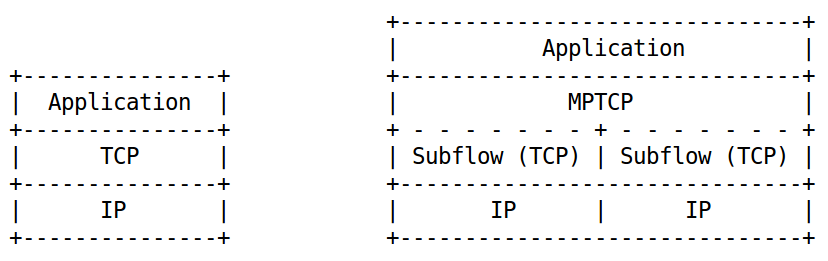
\includegraphics[width=0.75\textwidth]{images/stack}
\caption{The TCP and MPTCP protocol stacks}
\label{fig:stack}
\end{figure}

The choice of working at the transport layer was indeed the only available option. Within that option, the choice of maintaining TCP as the fundamental operating protocol for MPTCP was still straightforward for similar compatibility reasons; for this very purpose engineers decided to add all the required options for MPTCP inside the TCP \textit{Option} field in the TCP header. In this way, MPTCP-aware systems can process the MPTCP options for multipathing, but if a system that is not MPTCP-aware receives a MPTCP connection-request, it would simply discard the MPTCP options and treat such message as a plain TCP connection-request. 
MPTCP design maintains the behavior of the subflows to be compliant with regular TCP, while reassembling of data incoming from different paths is a process executed by the receiving host only. MPTCP subflows are indeed seen by middleboxes as regular and independent TCP connections carrying additional options. If security policies at the middleboxes is not too restrictive against unknown options, MPTCP-unaware nodes would still work with the new protocol.
For what regards applications, they don't need to be changed either since MPTCP would be inserted into the network stack at the operating system level: it would automatically split the data buffered from the application layer and send it through different subflows, according to the number of available endpoints at the connected hosts. Communication with the application layer can be performed through the old TCP APIs, even if MPTCP specific options can be used by upgraded user programs to take advantage of more advanced options in MPTCP.

A functional decomposition of MPTCP brings up four core functions the protocol offers:
\begin{itemize}
  \item \textit{Path management}: MPTCP has to provide a mechanism to detect and use multiple paths between two hosts;
  \item \textit{Packet scheduling}: MPTCP fragments the byte stream received from the application in order to transmit it through different subflows, adding the required sequenced mapping used to reconstruct the same byte stream at receiver. This function of MPTCP adopts the information from the path management component to exploit the different paths;
  \item \textit{Subflow interface}: as mentioned multiple times, MPTCP uses TCP to send data in a single subflow;
  \item \textit{Congestion control}: a congestion control mechanism at the MPTCP connection layer is needed to make sure that MPTCP wouldn't starve a singlepath TCP flow in a shared bottleneck. The congestion control component is the way MPTCP schedule segments at the various subflows, also taking into account the scheduling rate.
\end{itemize}

The previous functions of MPTCP are implemented internally at each host and they use a relatively compact set of TCP options to operate between two hosts. Technically, there is only a single generic MPTCP option, to which has been assigned the value 30 as the TCP "Option-Kind" identifier; at a lower level it is possible to identify a set of eight MPTCP option subtypes, each identified by a 4-bit value (this classification, reported in figure \ref{fig:MPTCP_options}, references to \rfc{6824}). 

\begin{figure}[!htb]
\centering
\includegraphics[width=0.75\textwidth]{images/MPTCP_options}
\caption{The set of MPTCP options [RFC-6824]}
\label{fig:MPTCP_options}
\end{figure}

\subsection{Control plane}
The control plane for MPTCP takes into consideration all the options used in MPTCP to handle connection initiation, addition and removal of subflows, priority assignment to specific subflows, error handling via 'fallback' mechanism. These options are reported in the following subsections, adopting as reference documentation the \rfc{6824}.

\subsubsection{MP\_CAPABLE}
The connection initiation of an MPTCP connection is very similar to the standard TCP initial three-way handshake, involving a SYN, SYN/ACK and ACK exchange on a single path between host A and host B. In a regular TCP connection establishment these three packets are used to guarantee that both hosts have received an acknowledgment of the connection and also to exchange the two random initial sequence numbers that will be used to acknowledge data delivery for the two directions of the connection. Despite working as regular TCP packets, if MPTCP is enabled the SYN packet from host A will have a MP\_CAPABLE option in the \textit{Options} field of the TCP header; if the receiver host B is not MPTCP-compatible it will simply discard the MP\_CAPABLE option and proceeds instantiating a regular TCP connection.
In case both hosts are MPTCP-compatible, the MP\_CAPABLE option is inserted in the three packets of the initial handshake for two purposes: advertise that both hosts are indeed MPTCP-compatible and allow them to exchange two 64-bit keys (Key-A and Key-B), according to the scheme in figure \ref{fig:mpcapable}.

\begin{figure}[!htb]
\centering
\includegraphics[width=0.75\textwidth]{images/mpcapable}
\caption{MPTCP connection initiation}
\label{fig:mpcapable}
\end{figure}

These keys are sent in clear inside the MP\_CAPABLE option only during the initial handshake and their purpose is to identify a specific MPTCP connection within a host (useful when associating a new subflow to an existing MPTCP connection, for example) and to provide shared security material that is used in MPTCP for authorization mechanisms (more on this later in this section). The \textit{Option} field in the TCP header can only be 40 bytes long, and it is not reserved to MPTCP only. For this reason it is of primary importance to keep the amount of MPTCP related metadata as low as possible. In fact, the original 64 bit keys are exchanged only during initial handshake; subsequently, shorter 32 bit tokens (Token-A and Token-B) derived from such keys will be used to address a specific MPTCP connection, even if this procedure requires additional checks in case of collisions with other tokens already assigned to other MPTCP connections in the same machine. Therefore, an implementation will require a mapping from each token to the corresponding connection, and in turn to the keys for the connection.


Regarding the hashing algorithm used to produce the tokens, this can be negotiated by using a portion of the flag bits inside the MP\_CAPABLE option. In this paper, the SHA1 (and HMAC-SHA1 in case a key element is needed) is considered [ref to SHA1]. Note that the SHA1 algorithm produces a 160-bit / 20-octet resulting value, that is then truncated to its leftmost 32 or 64 bits according to the different cases in the MPTCP operations.

\begin{figure}[!htb]
\centering
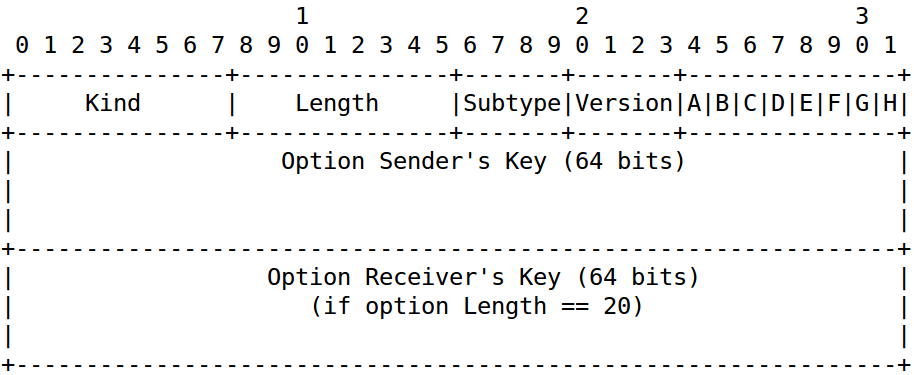
\includegraphics[width=0.75\textwidth]{images/opt_capable}
\caption{MP\_CAPABLE option}
\label{fig:opt_capable}
\end{figure}

\subsubsection{MP\_JOIN}
Suppose that after the first subflow is operational host A initiates a new subflow between one of its addresses and one of host B's addresses (figure \ref{fig:mptcpauth}). Host A sends a TCP SYN packet to host B containing the MP\_JOIN option, which includes Token-B (the token derived B's key) and a nonce value used to prevent replay attacks. An additional field in the MP\_JOIN option is called Address ID, an identifier for the original addresses in use within a single MPTCP connection; this additional value allows to refer to a specific subflow without the need to use the addresses as identifiers, which is very useful when middleboxes like NATs alter the IP header during the transit of the packets.

At the lower layers of the network, the SYN packet sent in this way looks like a legitimate request from host A to initiate a new TCP connection with host B, being the SYN packet the first of the regular TCP initial handshake. Host B treats such packet as a new MPTCP subflow request, and it uses the Token-B in the packet to associate the request to the specific ongoing MPTCP connection with host A.

The handshake flow for MP\_JOIN includes HMAC values for authentication purposes, and it is structured as follow:
\begin{itemize}
  \item Token-B is added in the SYN packet from host A to host B in order to address a specific MPTCP connection; a random nonce (R-A) is also sent along;
  \begin{figure}[!htb]
\centering
\includegraphics[width=0.75\textwidth]{images/opt_join1}
\caption{MP\_JOIN option - SYN}
\label{fig:opt_join1}
\end{figure}
  \item Host B processes the request and sends back a truncated HMAC value calculated by using as \textit{key} the concatenation of Key-B followed by Key-A, and as the \textit{message} the concatenation of a new nonce computed at host B (R-B) and the one received from host A (R-A). R-B is also added to the packet, since it is needed by host A in the next step;
\begin{figure}[!htb]
\centering
\includegraphics[width=0.75\textwidth]{images/opt_join2}
\caption{MP\_JOIN option - SYN/ACK}
\label{fig:opt_join2}
\end{figure}
  \item The last ACK form host A to host B only has to contain the HMAC calculated using as key the concatenation of Key-A and Key-B, and as message the concatenation R-A and R-B. This time, the HMAC value is sent in its full length of 160-bit.
\begin{figure}[!htb]
\centering
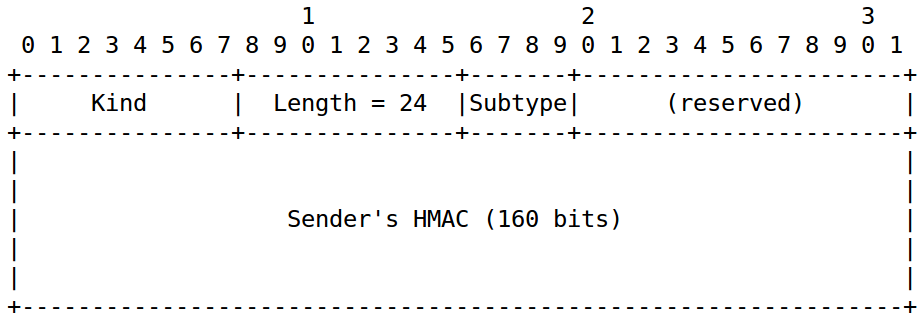
\includegraphics[width=0.75\textwidth]{images/opt_join3}
\caption{MP\_JOIN option - ACK}
\label{fig:opt_join3}
\end{figure}
  \item Note that the HMAC in the ACK packet from host A to host B has to be acknowledged for the subflow to be finally established. This because the third ACK is the only packet where the HMAC from host A is sent, and it has to be acknowledged or retransmitted is the fourth ACK from host B is not received.
\end{itemize}

These HMAC values are used to authenticate the participants in the subflow establishment, since both have to know the keys for the MPTCP connection. If the creation of the new subflow is not possible because A sends an unknown Token-B to host B or the HMAC material exchanged is not recognized by either hosts or the SYN/ACK received at host A misses the MP\_JOIN option, then the operation is stopped sending a TCP RST.


If everything works properly, the entire procedure of instantiating a MPTCP connection and add a subflow is represented with the example in figure \ref{fig:mptpcauth}. 

\begin{figure}[!htb]
\centering
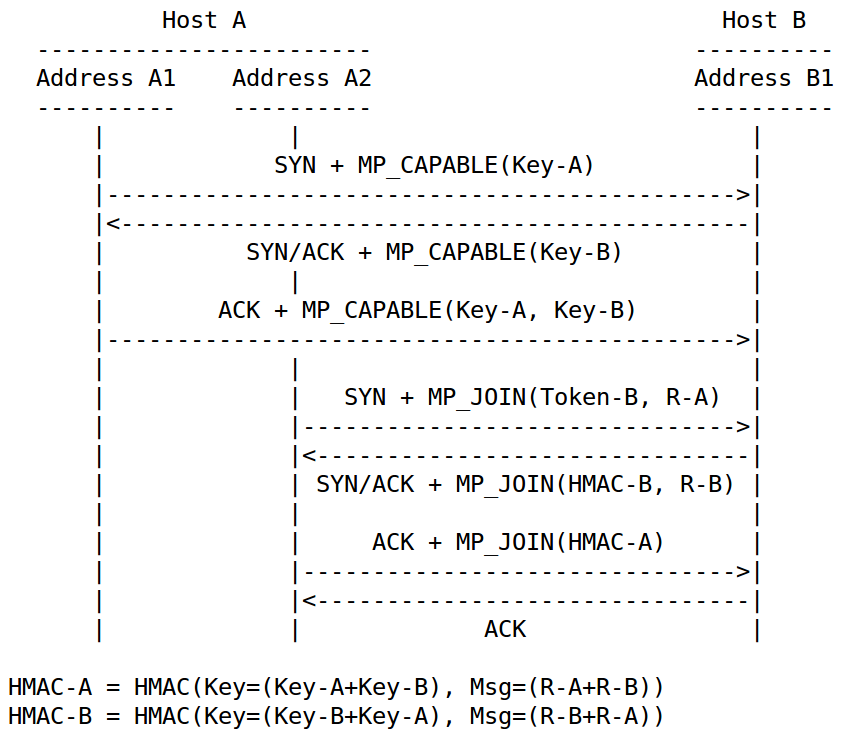
\includegraphics[width=0.75\textwidth]{images/mptcpauth}
\caption{MPTCP authentication example}
\label{fig:mptcpauth}
\end{figure}


\subsubsection{ADD\_ADDR}
Even if a host can directly instantiate a new subflow using the MP\_JOIN option as previously described, another possibility is for the host to advertise an available address to the other machine, thus allowing the latter to instantiate the subflow.
This functionalities can be useful, for example, in a typical client-server Web configuration in which only the client is allowed to open new connections with the server: if a new interface becomes available at the server, it can dynamically advertise it to the client which in turns can send the SYN+MP\_JOIN packet for subflow initiation.


This functionality is provided in MPTCP by the ADD\_ADDR option, that indeed contains the additional address (and, optionally, port) to be advertised. The option also includes the previously mentioned Address ID value, that has to uniquely address the address to the sender (within the same MPTCP connection).


The ADD\_ADDR option is treated as a soft component of the overall architecture, with no need to be sent reliably and/or be acknowledged by the receiver. The option can be added to any packet in the MPTCP connection if there is enough space in the \textit{Option} field of the TCP header, with no guarantee that such option will be received or that the receiver will indeed use the advertised information to start a new subflow. This low priority assigned to ADD\_ADDR is reasonable since the malfunctioning of this option would not break the overall data transmission, but it might only cause a missed opportunity for better multipath exploitation. For similar reasons, there is no need to ensure a proper ordering for ADD\_ADDR and REMOVE\_ADDR at the receiver (REMOVE\_ADDR, explained in the following subsection, is similar to ADD\_ADDR but it indicates which subflow to shut down instead). Albeit the typical TCP validity test will be performed before inspecting the ADD\_ADDR option.

The content of the ADD\_ADDR option is shown in figure \ref{fig:addaddropt}. The IPVer indicates if the advertised address is of kind IPv4 or IPv6, while the other fields contain the Address ID, Address and optional port as previously stated.

\begin{figure}[!htb]
\centering
\includegraphics[width=0.75\textwidth]{images/addaddropt}
\caption{ADD\_ADDR option}
\label{fig:addaddropt}
\end{figure}

\subsubsection{REMOVE\_ADDR}
If an address becomes unavailable during a MPTCP connection, the affected host should announce this so that any subflow currently using that address can be terminated. For security purposes, when a REMOVE\_ADDR is received, a test is performed to make sure that the address is not available anymore, by sending a TCP keepalive on the path.
The Address ID is used to identify the path to be shut down, so that no explicit address is needed (and no address is indeed present in the REMOVE\_ADDR option), and the option would work through NATs as well. 
A subflow that is working properly must not use this option to close the connection, but a FIN exchange similar to regular TCP is performed instead.

\begin{figure}[!htb]
\centering
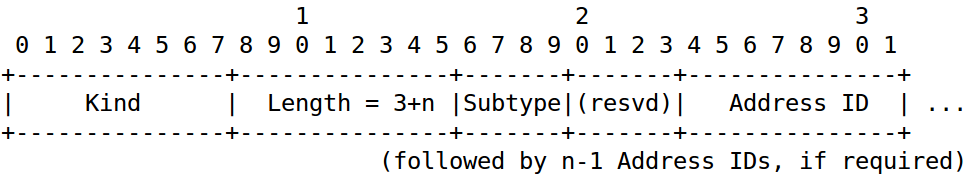
\includegraphics[width=0.75\textwidth]{images/opt_remove}
\caption{REMOVE\_ADDR option}
\label{fig:opt_remove}
\end{figure}



\subsubsection{MP\_FASTCLOSE}
This option can be thought as the MPTCP-level counterpart of the RST signal for the TCP connections: it permits the abrupt closure of the whole MPTCP connection. The RST signals couldn't trigger such behavior, since they are confined to work against a single TCP flow (i.e. MPTCP subflow).

This option can be sent by host A to trigger MPTCP closure at host B. In this case, MP\_FASTCLOSE must contain the value of Key-B. When host B receives the option through one of the subflows, it will send a TCP RST answer via the same subflow and then tears down all the subflow. Host A is waiting for the TCP RST answer from host B before tearing down all the subflows. This generic behavior might change slightly if both hosts send an MP\_FASTCLOSE at the same time, or if the awaited TCP RST signal is not received within a certain timeout (these would trigger a limited number of retransmissions for this option).

\begin{figure}[!htb]
\centering
\includegraphics[width=0.75\textwidth]{images/opt_fastclose}
\caption{MP\_FASTCLOSE option}
\label{fig:opt_fastclose}
\end{figure}

\subsubsection{MP\_FAIL}
There are various cases in which things might go wrong for a MPTCP connection, and the right procedure to handle such cases is to 'fall back', meaning either falling back to regular TCP or removing the subflow generating the issue. The first solution we saw already for the MP\_CAPABLE case, where TCP fall back is guaranteed in case a host is not MPTCP compatible. Similarly, subflow addition will be blocked if anything goes wrong in the MP\_JOIN packets' exchange procedure. However, there are other cases in which problems occur after this initiation phases, on regular packets.


As explained in section [ref to section "Data plane"], data acknowledgment with MPTCP requires a DSS option present in the ACK packets. If that option is missing, the path is not considered MPTCP capable. The consequences are different according to the subflow: if the affected path is the first instantiated with the MP\_CAPABLE option then it must fall back to regular TCP; any other subflow showing such problem would be closed with a RST. 


Fallback can be required at any point during the connection if a middlebox modifies the data stream. This case would be detected thanks to the checksum properties of MPTCP data transfer. If checksum fails, all data from the failing segment onwards cannot be trusted anymore. When this happens to a subflow, that has to be immediately closed with a RST and a MP\_FAIL option that indicates the data sequence number that failed the checksum. Such option indeed contains a single main field storing the full 64-bit sequence number. The receiver can then avoid to acknowledge untrusted data, that will be sent again through a different subflow following the retransmission features of the data plane part of the MPTCP protocol. After the fallback to regular TCP, it is mandatory not to revert back to MPTCP later on in the connection.


\begin{figure}[!htb]
\centering
\includegraphics[width=0.75\textwidth]{images/opt_fail}
\caption{MP\_FAIL option}
\label{fig:opt_fail}
\end{figure}

\subsubsection{MP\_PRIO}
It is possible to indicate if a path has to be used regularly or just as backup in case there no other available regular paths. This preference can be advertised at subflow creation via a flag in the MP\_JOIN option, but it is also possible to signal a priority change during the whole time of the MPTCP connection. In fact, it is enough to send the MP\_PRIO option to the targeted subflow to switch priority, to signal the other host about the change; it is also possible to add an Address ID to the option to target all the subflows using the addresses associated to such Address ID. This option is only sent from the receiver to the sender, even if the sender can discard such priority preference for any reasons. 


\begin{figure}[!htb]
\centering
\includegraphics[width=0.75\textwidth]{images/opt_prio}
\caption{MP\_PRIO option}
\label{fig:opt_prio}
\end{figure}

\subsection{Data plane}
This part concerns all the MPTCP options used to manage the data flow in a MPTCP connection, including how the byte stream is subdivided into different subflow and how the original order of the packets is provided at the receiver.

\subsubsection{DSS option}
In order for the receiver to reassemble the correct data stream in MPTCP, a specific option called DSS is used. This option contains the data mapping and Data ACK: data mapping is used to map the sequence space at each subflow (which is independently handled by the TCP protocol) to the overall sequence space at connection level; Data ACK is the procedure to acknowledge data receipt at connection level in MPTCP.
The DSS option can also signal the equivalent of a TCP FIN for the overall MPTCP connection, meaning that the current mapping covers the final data from the sender (figure \ref{fig:mptcp_fin}). 

\begin{figure}[!htb]
\centering
\includegraphics[width=0.75\textwidth]{images/mptcp_fin}
\caption{Closing a MPTCP connection}
\label{fig:mptcp_fin}
\end{figure}

This option might also include the checksum field to perform integrity checks on the payload (if this was enabled when instantiating the connection via the MP\_CAPABLE option).
DSS is indeed a versatile packet, whose per-packet behavior is mainly defined by the appropriate flags (figure \ref{fig:opt_dss}). 

Regarding the data sequence mapping in MPTCP, the general idea is to maintain TCP-compliant and independent sequence numbers for the single subflows, while using a mapping functionality at the MPTCP-level, provided by the DSS option, to properly rearrange the data at the receiver at guarantee in-order and reliable overall transmission as in the case of legacy TCP. The alternative approach would have been to have a single MPTCP-level sequence number used for the entire set of subflows, meaning that a single subflow inspected by middleboxes at the network infrastructure would look like a TCP connection with holes in the payload delivery; this could trigger unwanted behaviors that would be against the compatibility goals towards the current networks.


The DSS option achieves data sequence mapping with the combination of three fields: for a certain number of bytes (indicated in the \textit{Data-Level Length field}, and starting from the reported subflow sequence number (\textit{Subflow Sequence Number} field), the TCP-level sequence maps to the MPTCP-level sequence with starting value indicated in the \textit{Data sequence number} field.
The \textit{Data ACK} field works as regular TCP ACK value, but it refers to the MPTCP-level acknowledgment of the received data. Note that subflow-level acknowledgement is still provided by regular TCP, but a second acknowledgement mechanism at connection-level is desired, since there might cases in which data that has been acknowledges at the subflow-level can be discarded in the buffers before reaching the application. By following the core principles of MPTCP, retransmission of packets can occur at different paths.

\begin{figure}[!htb]
\centering
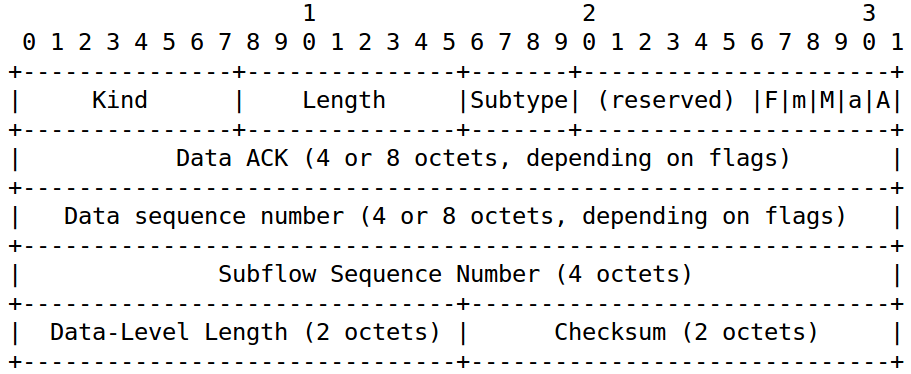
\includegraphics[width=0.75\textwidth]{images/opt_dss}
\caption{DSS option}
\label{fig:opt_dss}
\end{figure}

\section{MPTCP deployment}
Despite the big effort in designing a protocol compliant with strict compatibility requirements, assuring correct functioning in all the current network scenarios is not a viable possibility for MPTCP. The main problematics are related to unwanted behavior of middleboxes processing unknown MPTCP packets, but that is not the only aspect currently limiting the deployment status of the new protocol. MPTCP has to guarantee the same levels of reliability, performance and security of regular TCP (including the cases in which the fallback mechanism is adopted to switch to plain TCP). Moving further away from technical details, deployment of such a protocol would have a big impact on the business models currently available for Internet access provisioning, and it is very important to analyze the relation between costs and benefits that MPTCP would bring to each and every group of MPTCP stakeholders.


The success of MPTCP strongly depends on its deployment, and its deployment strongly depends on endpoints. As previously mentioned, there is conceptually no need for technical modifications at the intermediate infrastructure to make MPTCP available at the end users, the latter being the ones directly accessing the biggest part of MPTCP benefits as described in section [add MPTCP benefits section]. Nevertheless, connectivity providers still represent an important part of the entire set of stakeholders that might benefit from MPTCP wide adoption: MPTCP can directly improve resource utilization and congestion bottlenecks within the overall infrastructure, but it can also be seen as an enabler of new business models for the ISPs, since end users might show an increase interest in multihoming solutions [\href{https://books.google.de/books?id=ECBxhiURlKYC&pg=PA23&lpg=PA23&dq=mptcp+deployment&source=bl&ots=_cvPxxdH6K&sig=P5AlF9bU_iE3C63HfXvgD77tUg8&hl=en&sa=X&ved=0ahUKEwi0wMnuscfKAhUB1hQKHT0cARsQ6AEIUzAI#v=onepage&q&f=false}{href}]. End users and ISPs feedback for MPTCP would drive the interest of infrastructure vendors to better support the protocol or not. 
Yet another case study involves data infrastructure maintainers and the benefits that MPTCP can bring to data centers of today as well as the possibilities enabled by MPTCP for the design of the data centers of the future [\href{http://conferences.sigcomm.org/sigcomm/2011/papers/sigcomm/p266.pdf}{href}].


The following sections disregard business motives of MPTCP adoption and focus on some core technical aspects of the protocol deployment, considering middleboxes compatibility, OS implementations status and finally an overview of the current rate of adoption and future trends.

\subsection{Middleboxes compatibility}
The Internet at its core was designed to provide end-to-end connectivity across an infrastructure of interconnected routers. Nevertheless, the growing rate of adoption and increasing complexity of the Internet brought up a wide set of new requirements inherent the intermediate stages of the communication rather then the end-hosts. Such requirements include the need to instantiate protection techniques against potential attacks, more flexibility in content delivery, caching for more efficient communication; they can even be more specific, like the need to rapidly overcome the previously mentioned IPv4 addresses depletion. Middleboxes are pieces of equipment that operate on the network traffic to meet these requirements. The most common middleboxes are NATs, proxies and firewalls, but nowadays there is a huge variety of deployed middleboxes that inevitably break the end-to-end principle of the Internet. Despite their usage is often required, they are more or less intrusive at different layers of operation (according to where they operate within the OSI architectural model), thus causing malfunctioning of many protocols, and MPTCP is no exception. Middleboxes can indeed inspect packets, re-route them, drop them, split them into multiple fragments, and even modify single fields in packets' headers (like rewriting sequence number or removing TCP options) as well as change their payload.


The various operations and purposes of middleboxes are many and often mixed together to achieve more complex policies, and it is also very common that different kind of operations are performed inside the same physical machine. Despite this, it is possible to define a set of most common distinct middleboxes' operations [\href{https://queue.acm.org/detail.cfm?id=2591369}{href}]. 

\subsubsection{Firewalls}
A simple example can be the case of a standard firewall that is not MPTCP-aware and its default policy is set to "Deny". In this case, all the traffic is blocked unless the set of custom rules configured in the firewall explicitly allows a specific typology of packets. In this case, specific for MPTCP must be added to support the new protocol, and this might cause a considerable effort for network maintainers. For example, it is often not straightforward to operate on legacy firewall configurations for big companies with many access points.
A more subtle problem with firewalls might be derived by the fact that they can sometimes manipulate the sequence numbers of a TCP connection, thus moving the sequence number space with respect to the initial value in use by the end-hosts. This feature has been introduced in the past to improve security, but the concept can disrupt MPTCP mapping between subflow sequence number and MPTCP-level sequence number. To avoid such problems, MPTCP is designed so that the mapping in the DSS option is using relative values compared to the initial sequence number and functioning is not jeopardized but changes of the absolute values performed by the firewalls.

\subsubsection{NATs}
Another ubiquitous piece of equipment is the "Network Address Translation" (NAT). As the name suggests, NATs modify the IP addresses within the packets on their way towards the destination. The main purpose is to group addresses of an internal private network and map them to a single public address before forward the traffic to the Internet. NATs are also able to redirect the response from the Internet to the right host in the internal network.
This procedure became very common with the depletion of IPv4 addresses, since in many cases the address space assigned to a outer portion of the Internet is not large enough to cover the number of hosts willing to acquire connectivity. 
NATs turned out to be a very effective way to temporarily solve the problem of IPv4 addresses, but their mode of operation is intrusive at the network and transport layer, since the IP addresses are not fixed anymore.
For example, even if NATs use internal tables to keep track of the mappings and are able to redirect replies from the external network to the right internal host, it is no more possible for the external hosts to instantiate a new connection with a specific host residing behind a NAT. This is true also in MPTCP, such that a server often cannot open a new subflow with a client if the latter is behind a NAT, even if a valid MPTCP session between client and server is already active. This is one of the main use cases in which an ADD\_ADDR message can be sent on live subflows in order to trigger a new subflow connection request from the other side.
Moreover, to cope with NATs that might be operational on the paths and might change the source address of the packets, MPTCP refers to addresses by using an Address ID, as previously mentioned in the section [add ref to control plane]. 

\subsubsection{Segment splitting and coalescing}
There are middleboxes that split segments on the Internet as required by the MTU (maximum transmission unit). This means that the payload of a single TCP packet can be scattered across multiple smaller TCP packets and regrouped back together by using the appropriate TCP fields in the header. This operation usually copies TCP options unchanged into each of the smaller packets that are generated. By simply adopting data-sequence numbers in a MPTCP option, the receiver might receive different packets with the same data-sequence numbers and it would be unable to reconstruct the original data. MPTCP takes care of segment splitting and coalescing by mapping the subflow-level TCP sequence number with the MPTCP-level sequence, by providing both the beginning (with respect to the subflow sequence number) and the end of the of the data-sequence number [section about DSS].

\subsubsection{Application-level gateways}


\subsection{Implementations}
Despite the previously described problematics, MPTCP is a big bet in the IETF community and many implementations have been developed for the most common OSes, listed in this section (with some history notions).

\subsection{Deployment status}
It should be interesting for the reader to go through some examples of real world's scenarios in which MPTCP is used successfully. Here it is possible to cite some important achievements related to MPTCP (for example the highest throughput ever reached with the new protocol).
If available, it would be also good to show some graphs about MPTCP adoption rate or similar.